\documentclass[12pt,a4paper,oneside,brazil,chapter=TITLE,section=TITLE]{abntex2}

\usepackage[T1]{fontenc}
\usepackage[utf8]{inputenc}
\usepackage[brazil]{babel}
\usepackage{lmodern}
\usepackage{microtype}
\usepackage{graphicx}
\usepackage{amsmath,amssymb}
\usepackage{booktabs}
\usepackage{float}
\usepackage{listings}
\usepackage{xcolor}
\usepackage{caption}
\usepackage{subcaption}
\usepackage{geometry}
\usepackage{abntex2cite}
\usepackage{url}
\usepackage{algorithm}
\usepackage{algpseudocode}

\geometry{top=3cm,bottom=2cm,left=3cm,right=2cm}

\lstset{
  basicstyle=\ttfamily\footnotesize,
  breaklines=true,
  keywordstyle=\color{blue!70!black}\bfseries,
  commentstyle=\color{green!50!black}\itshape,
  stringstyle=\color{red!60!black},
  numbers=left, numberstyle=\tiny\color{gray},
  numbersep=6pt,
  frame=single, rulecolor=\color{gray!40},
  tabsize=2,
  showstringspaces=false,
}
\lstdefinestyle{matlab}{language=Matlab}

\titulo{Projeto 8 -- Limiariza\c{c}\~ao Global (\textit{GlobalThresholding})}
\autor{Matheus Serr\~ao Uch\^oa}
\local{Manaus -- AM}
\data{maio de 2026}
\instituicao{%
  Universidade Federal do Amazonas -- UFAM\\
  Instituto de Computa\c{c}\~ao -- IComp\\
  Disciplina: Processamento Digital de Imagens}
\tipotrabalho{Relat\'orio de Atividade}
\preambulo{Relat\'orio referente ao Projeto~8 da disciplina de
  Processamento Digital de Imagens, abordando o algoritmo de
  limiariza\c{c}\~ao global iterativa e sua aplica\c{c}\~ao
  na imagem \textit{rice-shaded.tif}.}

\makeatletter
\hypersetup{
  pdftitle={\@titulo},
  pdfauthor={\@autor},
  colorlinks=true,
  linkcolor=blue!60!black,
  citecolor=green!50!black,
  urlcolor=blue
}
\makeatother

\begin{document}

%% ================================================================
%% CAPA
%% ================================================================
\begin{capa}
  \center
  
\includegraphics[width=3cm]{ufam_logo.png}\\[0.5cm]
  {\large\bfseries Universidade Federal do Amazonas}\\
  {\large Instituto de Computa\c{c}\~ao -- IComp}\\[1cm]
  \vfill
  {\LARGE\bfseries Processamento Digital de Imagens}\\[0.4cm]
  {\Large\bfseries Projeto 8}\\[0.3cm]
  {\large Limiariza\c{c}\~ao Global (\textit{GlobalThresholding})}\\
  \vfill
  {\large Matheus Serr\~ao Uch\^oa}\\[0.5cm]
  {\large Manaus -- AM, maio de 2026}
\end{capa}

%% ================================================================
%% FOLHA DE ROSTO
%% ================================================================
\begin{folhaderosto}
  \begin{center}
    {\large\bfseries Matheus Serr\~ao Uch\^oa}\\[2cm]
    {\LARGE\bfseries Projeto 8 -- Limiariza\c{c}\~ao Global}\\[1.5cm]
  \end{center}
  \begin{flushright}
    \begin{minipage}{9cm}
      \small
      Relat\'orio apresentado como atividade avaliativa da disciplina
      de Processamento Digital de Imagens do Instituto de Computa\c{c}\~ao
      da Universidade Federal do Amazonas.
    \end{minipage}
  \end{flushright}
  \vfill
  \begin{center}{\large Manaus -- AM, maio de 2026}\end{center}
\end{folhaderosto}

%% ================================================================
%% RESUMO
%% ================================================================
\begin{resumo}
Este relat\'orio descreve a implementa\c{c}\~ao e avalia\c{c}\~ao
do algoritmo de limiariza\c{c}\~ao global iterativa para segmenta\c{c}\~ao
de imagens em n\'iveis de cinza.
Na Parte~(a), \'e implementada a fun\c{c}\~ao \texttt{globalThresh(f,~detT)}
em MATLAB, que escala automaticamente a imagem para o intervalo $[0,1]$,
estima um limiar inicial e itera at\'e a converg\^encia definida pelo
crit\'erio $\Delta T < \texttt{detT}$ (padr\~ao $= 0{,}01$).
Na Parte~(b), a fun\c{c}\~ao \'e aplicada \`a imagem
\textit{rice-shaded.tif} com os par\^ametros padr\~ao.
O limiar converge em apenas 4 itera\c{c}\~oes para $T \approx 0{,}441$,
por\'em o resultado apresenta erros de segmenta\c{c}\~ao nas regi\~oes
escuras da imagem, evidenciando a limita\c{c}\~ao fundamental da
limiariza\c{c}\~ao global: a incapacidade de lidar com ilumina\c{c}\~ao
de fundo n\~ao uniforme.
Na Parte~(c), diferentes valores de \texttt{detT} s\~ao explorados,
demonstrando que a escolha deste par\^ametro n\~ao resolve o problema,
pois o algoritmo converge para limiares praticamente id\^enticos
($\Delta T < 0{,}002$) independentemente de \texttt{detT}.

\vspace{0.5cm}
\noindent\textbf{Palavras-chave:}
Limiariza\c{c}\~ao global.
Segmenta\c{c}\~ao de imagens.
Fundo n\~ao uniforme.
Itera\c{c}\~ao.
\end{resumo}

\tableofcontents*
\cleardoublepage
\textual

%% ----------------------------------------------------------------
\chapter{Introdu\c{c}\~ao}
%% ----------------------------------------------------------------

A segmenta\c{c}\~ao de imagens consiste em dividir uma imagem em
regi\~oes significativas, separando objetos de interesse do fundo.
A limiariza\c{c}\~ao \'e a abordagem mais simples: dada uma imagem
$f(x,y)$ e um limiar $T$, a imagem segmentada \'e:
\begin{equation}
  g(x,y) = \begin{cases} 1 & \text{se } f(x,y) > T \\ 0 & \text{caso contr\'ario} \end{cases}.
\end{equation}

O desafio central \'e determinar automaticamente o limiar $T$ adequado.
O algoritmo de limiariza\c{c}\~ao global iterativa \cite{gonzalez2018}
estima $T$ a partir das m\'edias dos dois grupos (objeto e fundo),
iterando at\'e a converg\^encia.

Este relat\'orio est\'a estruturado em tr\^es partes correspondentes
\`as atividades do Projeto~8:
\begin{itemize}
  \item \textbf{Parte (a):} implementa\c{c}\~ao da fun\c{c}\~ao
        \texttt{globalThresh};
  \item \textbf{Parte (b):} aplica\c{c}\~ao em \textit{rice-shaded.tif}
        e discuss\~ao dos erros;
  \item \textbf{Parte (c):} avalia\c{c}\~ao do impacto do crit\'erio
        de parada \texttt{detT}.
\end{itemize}

%% ----------------------------------------------------------------
\chapter{Fundamenta\c{c}\~ao Te\'orica}
%% ----------------------------------------------------------------

\section{Algoritmo de Limiariza\c{c}\~ao Global Iterativa}

O algoritmo, descrito em \citeonline{gonzalez2018}, opera da seguinte
forma:

\begin{algorithm}[H]
\caption{Limiariza\c{c}\~ao global iterativa}
\begin{algorithmic}[1]
  \State Escale $f$ para $[0,1]$: $\hat{f} = (f - \min f) / (\max f - \min f)$
  \State $T \leftarrow \text{m\'edia}(\hat{f})$
  \Repeat
    \State $G_1 \leftarrow \{(x,y) : \hat{f}(x,y) > T\}$ \Comment{grupo objeto}
    \State $G_2 \leftarrow \{(x,y) : \hat{f}(x,y) \leq T\}$ \Comment{grupo fundo}
    \State $m_1 \leftarrow \text{m\'edia}(G_1)$, \quad $m_2 \leftarrow \text{m\'edia}(G_2)$
    \State $T_{\text{novo}} \leftarrow (m_1 + m_2) / 2$
    \State $\Delta T \leftarrow |T_{\text{novo}} - T|$; \quad $T \leftarrow T_{\text{novo}}$
  \Until{$\Delta T < \texttt{detT}$}
  \State \Return $g = (\hat{f} > T)$
\end{algorithmic}
\end{algorithm}

O algoritmo converge porque a sequ\^encia de limiares $T_k$ \'e
mon\'otona e limitada: cada itera\c{c}\~ao recalcula as m\'edias com
base na parti\c{c}\~ao atual, e o ponto fixo corresponde ao limiar
\'{o}timo para um modelo de mistura bimodal \cite{otsu1979}.

\section{Limita\c{c}\~ao: Fundo N\~ao Uniforme}

A limiariza\c{c}\~ao global pressup\~oe que a imagem possui histograma
bimodal bem definido, com um vale claro separando objeto e fundo.
Quando o fundo apresenta ilumina\c{c}\~ao gradiente (como em
\textit{rice-shaded.tif}), os pixels do fundo escuro e os pixels de
gr\~aos de arroz na regi\~ao escura podem ter intensidades sobrepostas,
tornando um \'unico limiar global inadequado \cite{gonzalez2018}.

Nesse caso, t\'ecnicas mais robustas como limiariza\c{c}\~ao local
adaptativa, corre\c{c}\~ao de ilumina\c{c}\~ao (\textit{background
subtraction}) ou o m\'etodo de Otsu por blocos s\~ao prefer\'iveis.

%% ----------------------------------------------------------------
\chapter{Implementa\c{c}\~ao}
%% ----------------------------------------------------------------

\section{Parte (a) -- Fun\c{c}\~ao \texttt{globalThresh}}

A fun\c{c}\~ao \texttt{globalThresh.m} implementa o algoritmo descrito
na Se\c{c}\~ao 2.1, com as seguintes decis\~oes de projeto:

\begin{itemize}
  \item A escala para $[0,1]$ \'e feita com base nos valores min/max
        reais da imagem, n\~ao em valores fixos como 0 e 255;
  \item Prot\'ege\c{c}\~ao contra grupos vazios ($G_1$ ou $G_2$);
  \item O valor padr\~ao \texttt{detT = 0.01} \'e compat\'ivel com a
        escala $[0,1]$, equivalendo a $\approx 1{,}96$ n\'iveis de cinza
        em uma imagem de 8 bits.
\end{itemize}

\begin{lstlisting}[style=matlab, caption={globalThresh.m -- n\'ucleo do algoritmo}]
function [g, T, iters] = globalThresh(f, detT)
  if nargin < 2, detT = 0.01; end
  f = double(f);
  f_scaled = (f - min(f(:))) / (max(f(:)) - min(f(:)));
  T = mean(f_scaled(:));
  iters = 0;
  while true
    iters = iters + 1;
    G1 = f_scaled(f_scaled >  T);
    G2 = f_scaled(f_scaled <= T);
    m1 = mean(G1); m2 = mean(G2);
    T_new = (m1 + m2) / 2;
    if abs(T_new - T) < detT, T = T_new; break; end
    T = T_new;
  end
  g = f_scaled > T;
end
\end{lstlisting}

%% ----------------------------------------------------------------
\chapter{Resultados e Discuss\~ao}
%% ----------------------------------------------------------------

\section{Parte (b) -- Aplica\c{c}\~ao em \textit{rice-shaded.tif}}

A Figura~\ref{fig:part_b_default} apresenta a imagem original, o
histograma normalizado com o limiar encontrado e a imagem segmentada.

\begin{figure}[H]
  \centering
  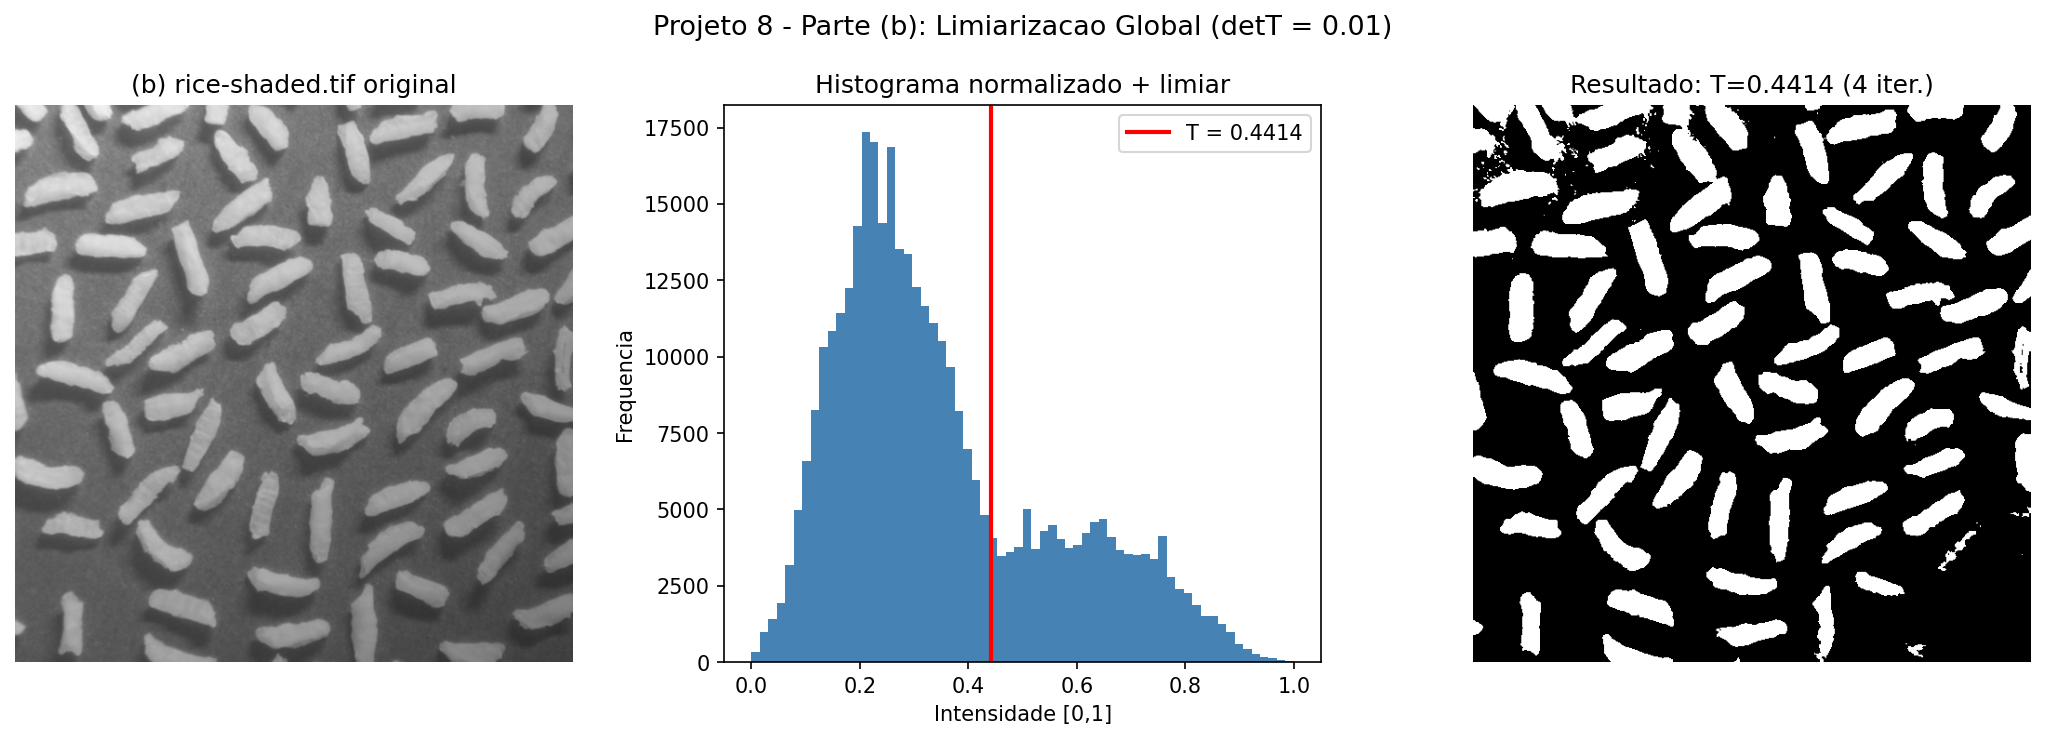
\includegraphics[width=\linewidth]{imgs_result/part_b_default.png}
  \caption{Parte (b): imagem original, histograma com limiar ($T = 0{,}4414$)
           e resultado da limiariza\c{c}\~ao global (\texttt{detT}~$= 0{,}01$,
           4~itera\c{c}\~oes).}
  \label{fig:part_b_default}
  \fonte{Elaborado pelo autor (2026).}
\end{figure}

O algoritmo convergiu em \textbf{4 itera\c{c}\~oes} para
$T = 0{,}4414$, equivalente a $\approx 135$ na escala original
$[47, 243]$. Aproximadamente 27,3\% dos pixels foram classificados
como objeto (gr\~aos de arroz).

\subsection{Erros de segmenta\c{c}\~ao e suas causas}

\noindent\textbf{Problema observado:} a imagem \textit{rice-shaded.tif}
possui fundo com ilumina\c{c}\~ao gradiente -- mais clara no centro e
mais escura nas bordas. Isso causa dois tipos de erro com um \'unico
limiar global:
\begin{enumerate}
  \item \textbf{Falsos negativos nas bordas escuras:} gr\~aos de arroz
        na periferia da imagem t\^em intensidade inferior ao limiar
        global e s\~ao classificados como fundo, desaparecendo da
        imagem bin\'aria.
  \item \textbf{Falsos positivos no centro claro:} pixels do fundo
        pr\'oximos ao centro, mais iluminados, podem superar o limiar
        e ser incorretamente classificados como gr\~aos.
\end{enumerate}

A Figura~\ref{fig:part_b_nonuniform} ilustra esse problema com perfis
horizontais em tr\^es linhas distintas da imagem.

\begin{figure}[H]
  \centering
  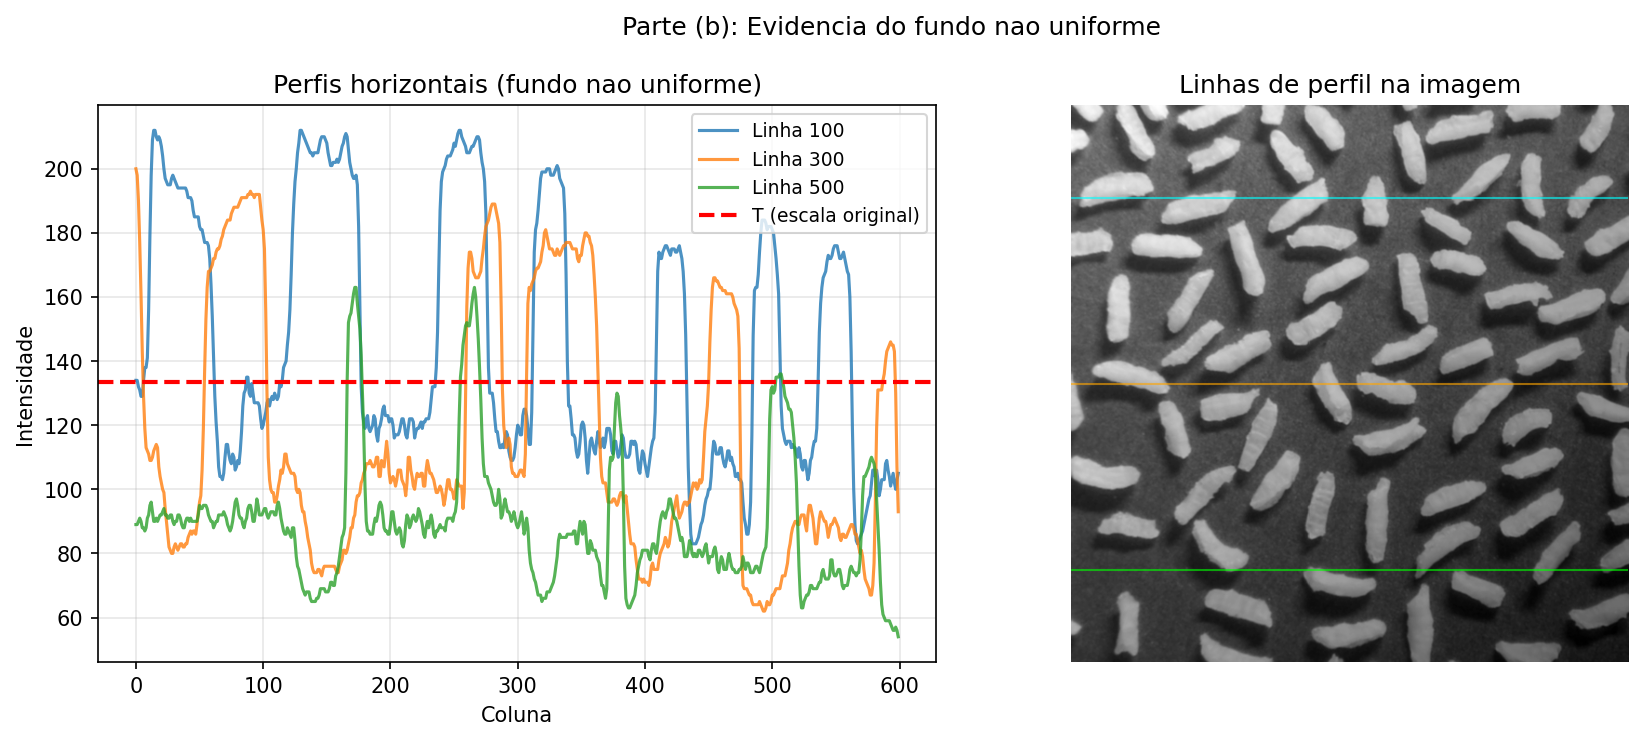
\includegraphics[width=\linewidth]{imgs_result/part_b_nonuniform_evidence.png}
  \caption{Perfis de intensidade horizontal em tr\^es linhas da imagem.
           O fundo na linha~100 (topo) \'e mais escuro que na linha~300
           (centro), criando sobreposic\~ao de intensidades objeto/fundo.}
  \label{fig:part_b_nonuniform}
  \fonte{Elaborado pelo autor (2026).}
\end{figure}

A Figura~\ref{fig:part_b_conv} confirma a r\'apida converg\^encia do
algoritmo, que estabiliza j\'a na 4\textordfeminine{} itera\c{c}\~ao.

\begin{figure}[H]
  \centering
  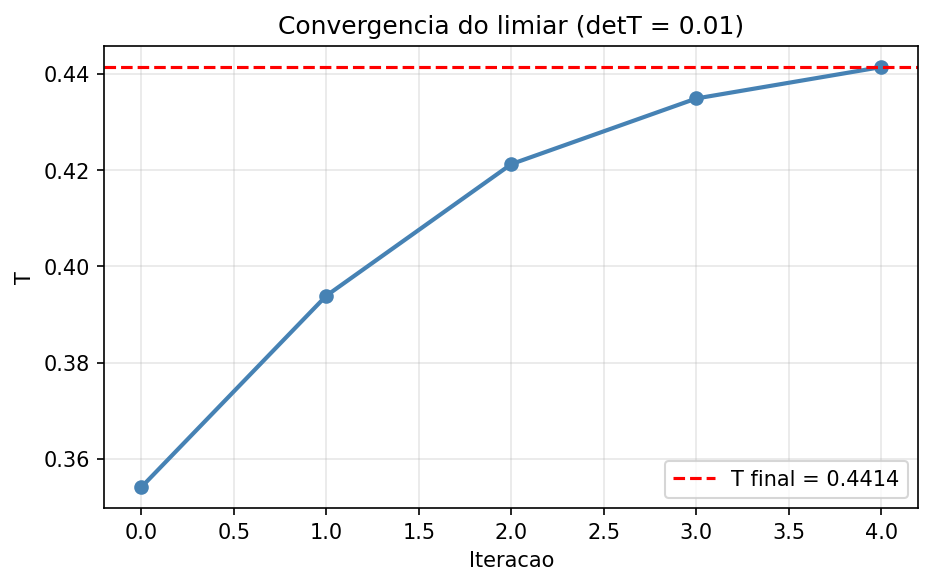
\includegraphics[width=0.6\linewidth]{imgs_result/part_b_convergence.png}
  \caption{Hist\'orico de converg\^encia do limiar $T$ para
           \texttt{detT}~$= 0{,}01$.}
  \label{fig:part_b_conv}
  \fonte{Elaborado pelo autor (2026).}
\end{figure}

\section{Parte (c) -- Impacto do crit\'erio de parada \texttt{detT}}

\noindent\textbf{Resposta \`a pergunta do enunciado:}
\textit{Outros valores de \texttt{detT} melhoram o resultado?}
\textbf{N\~ao.}

A Figura~\ref{fig:part_c_comparison} mostra os resultados para
$\texttt{detT} \in \{0{,}1;\; 0{,}01;\; 0{,}001;\; 0{,}0001\}$.

\begin{figure}[H]
  \centering
  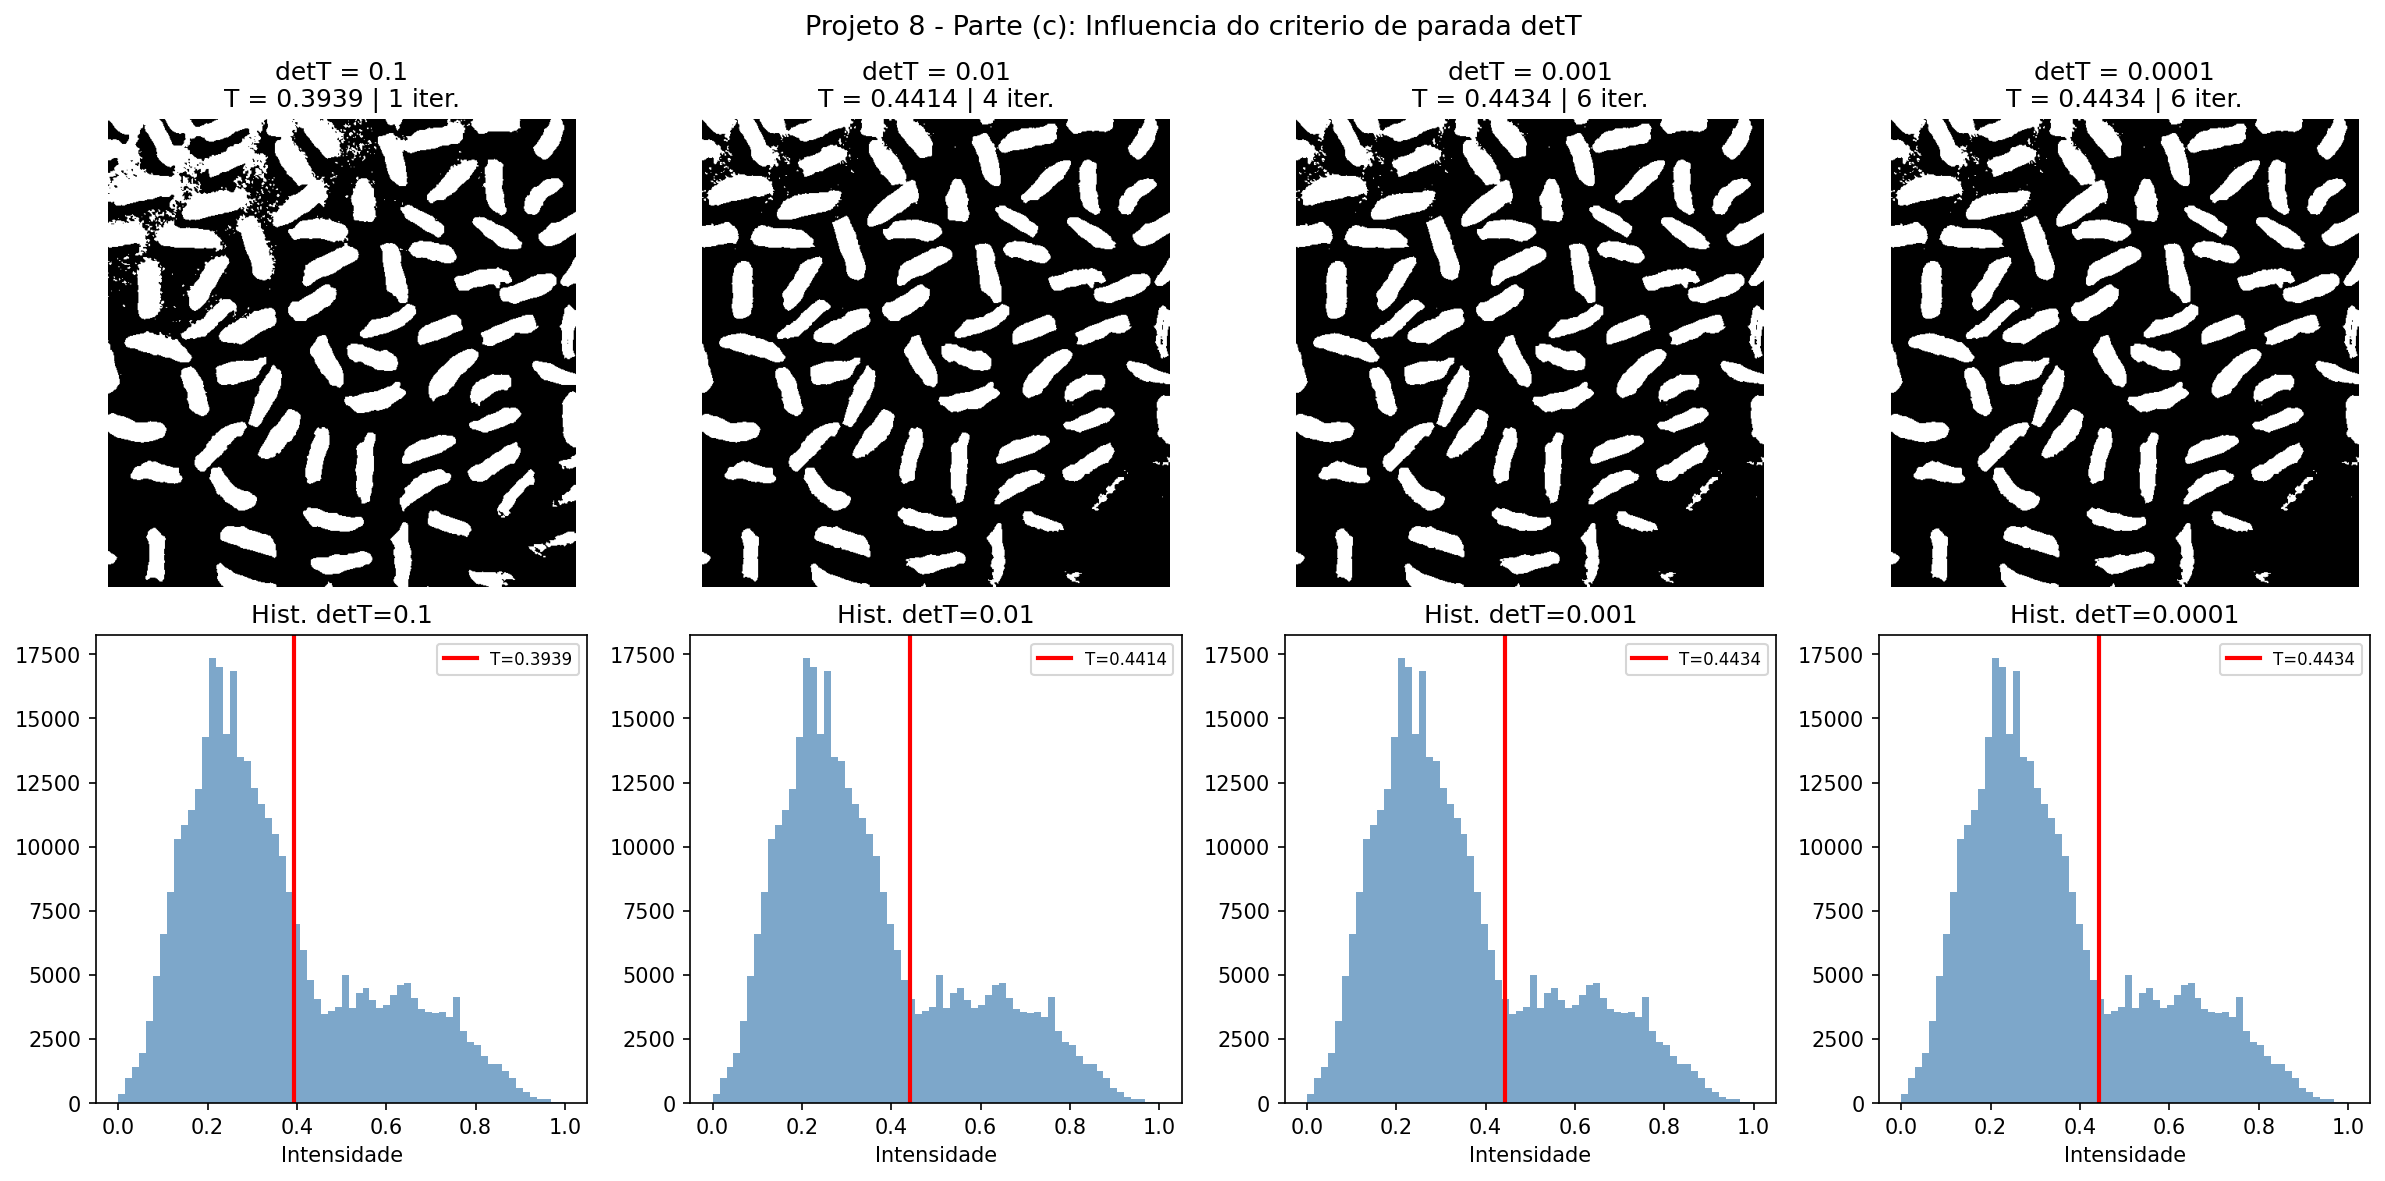
\includegraphics[width=\linewidth]{imgs_result/part_c_detT_comparison.png}
  \caption{Parte (c): resultados de limiariza\c{c}\~ao para quatro
           valores de \texttt{detT}. As diferen\c{c}as visuais entre
           os resultados com \texttt{detT}~$\leq 0{,}01$ s\~ao
           imperceptiveis.}
  \label{fig:part_c_comparison}
  \fonte{Elaborado pelo autor (2026).}
\end{figure}

\noindent\textbf{Justificativa:} como mostra a
Figura~\ref{fig:part_c_conv_all}, o algoritmo converge para limiares
praticamente id\^enticos independentemente de \texttt{detT}:

\begin{table}[H]
  \centering
  \caption{Limiar convergido e itera\c{c}\~oes para diferentes \texttt{detT}.}
  \label{tab:detT}
  \begin{tabular}{cccc}
    \toprule
    \texttt{detT} & $T$ convergido & Itera\c{c}\~oes & $\Delta T$ acumulado \\
    \midrule
    0,1000  & 0,3939 & 1 & -- (parada prematura) \\
    0,0100  & 0,4414 & 4 & 0,0475 \\
    0,0010  & 0,4434 & 6 & 0,0020 \\
    0,0001  & 0,4434 & 6 & $<0,0001$ \\
    \bottomrule
  \end{tabular}
  \fonte{Elaborado pelo autor (2026).}
\end{table}

\begin{figure}[H]
  \centering
  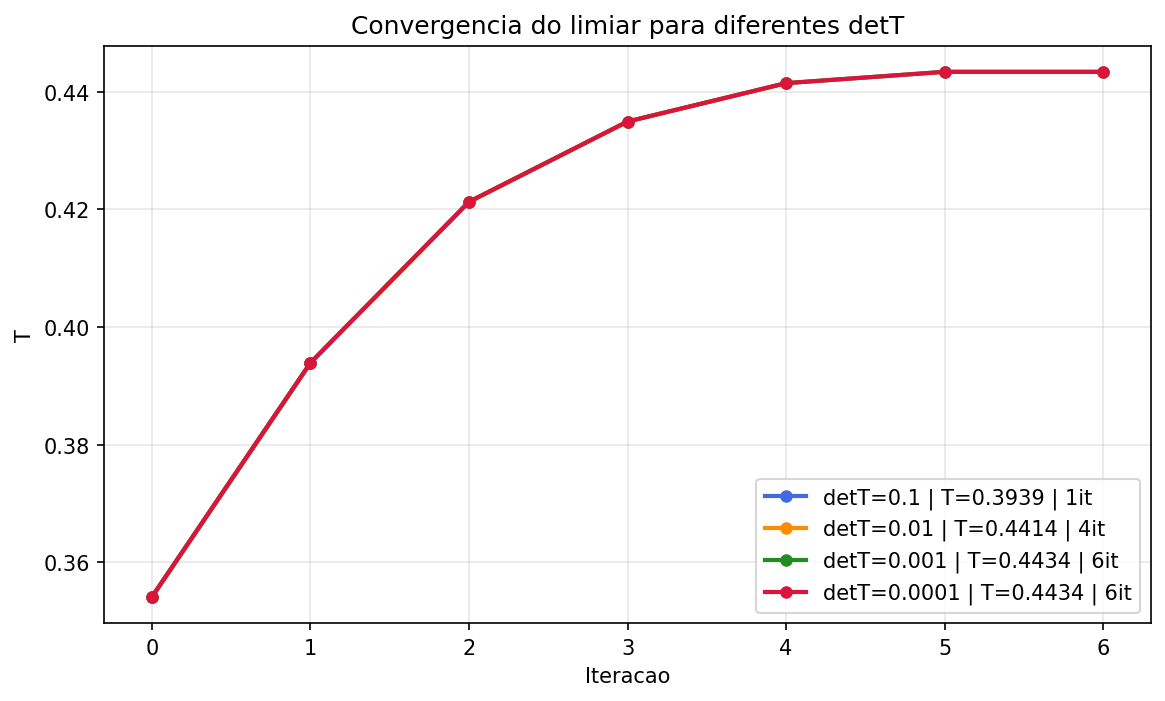
\includegraphics[width=0.8\linewidth]{imgs_result/part_c_convergence_all.png}
  \caption{Curvas de converg\^encia do limiar $T$ para todos os valores
           de \texttt{detT}. Exceto para \texttt{detT}~$= 0{,}1$
           (para prematuramente), todas as curvas convergem para
           $T \approx 0{,}443$.}
  \label{fig:part_c_conv_all}
  \fonte{Elaborado pelo autor (2026).}
\end{figure}

\noindent\textbf{Por que detT n\~ao resolve o problema?}
O par\^ametro \texttt{detT} controla apenas a precis\~ao de
converg\^encia do limiar, n\~ao a qualidade do limiar em si.
O algoritmo j\'a encontra o ponto fixo correto com
\texttt{detT}~$= 0{,}01$.
A causa raiz dos erros \'e estrutural: o pressuposto de ilumina\c{c}\~ao
uniforme \'e violado pela imagem \textit{rice-shaded.tif}.

Para resolver o problema seria necess\'ario, por exemplo:
\begin{itemize}
  \item \textbf{Corre\c{c}\~ao de ilumina\c{c}\~ao:} subtrair o fundo
        estimado (filtro morfol\'ogico tophat) antes da limiariza\c{c}\~ao;
  \item \textbf{Limiariza\c{c}\~ao adaptativa local:} calcular um limiar
        independente para cada bloco ou vizinhan\c{c}a da imagem.
\end{itemize}

%% ----------------------------------------------------------------
\chapter{Conclus\~ao}
%% ----------------------------------------------------------------

O algoritmo de limiariza\c{c}\~ao global iterativa foi implementado
com sucesso na fun\c{c}\~ao \texttt{globalThresh}, que escala a imagem
automaticamente para $[0,1]$ e itera at\'e a converg\^encia do limiar.
Os principais achados s\~ao:

\begin{enumerate}
  \item O algoritmo \'e eficiente: converge em 4--6 itera\c{c}\~oes
        para a imagem analisada;
  \item O limiar encontrado ($T \approx 0{,}443$) \'e est\'avel e
        praticamente independente de \texttt{detT} para valores
        $\leq 0{,}01$;
  \item Os erros de segmenta\c{c}\~ao em \textit{rice-shaded.tif}
        decorrem do gradiente de ilumina\c{c}\~ao do fundo, n\~ao do
        crit\'erio de parada;
  \item Alterar \texttt{detT} n\~ao melhora o resultado: a melhora
        real exigiria pr\'e-processamento (corre\c{c}\~ao de
        ilumina\c{c}\~ao) ou limiariza\c{c}\~ao adaptativa.
\end{enumerate}

\postextual
\bibliography{referencias_project8}

\end{document}
